\documentclass[12pt, letterpaper]{article}

\usepackage[english]{babel} % Sets the language and regional settings for English documents
\usepackage[utf8]{inputenc} % Allows the use of UTF-8 characters in the document
\usepackage[T1]{fontenc} % Specifies the font encoding
\usepackage[margin=2cm]{geometry} % Sets the page margins
\usepackage{makeidx} % Enables the creation of indexes
\usepackage{natbib} % Provides flexible bibliography support
\usepackage{url} % Allows the use of URLs
\usepackage{enumitem} % Customizes the appearance of lists
\usepackage{listings} % Provides syntax highlighting for code listings
\usepackage[dvipsnames]{xcolor} % Allows the use of colors
\usepackage{parskip} % Modifies paragraph spacing
\usepackage{graphicx} % Enables the inclusion of graphics
\usepackage{tikz} % Allows the creation of graphics and diagrams
\usepackage{float}
\usepackage{hyperref} % Enables the creation of hyperlinks
\usepackage{amsmath} % Provides additional math environments and commands
\usepackage{circuitikz} % Allows the creation of electrical circuits
\usepackage{adjustbox} % Adjusts the size of the circuit diagrams
\usepackage{arydshln} % Allows the use of dashed lines in tables

\usetikzlibrary{shapes.geometric, positioning}

\lstset{
	language=SQL,
	basicstyle=\ttfamily\small,
	keywordstyle=\color{blue},
	commentstyle=\color[rgb]{0,0.5,0},
	stringstyle=\color{red},
	numbers=left,
	numberstyle=\tiny\color{gray},
	stepnumber=1,
	numbersep=10pt,
	backgroundcolor=\color{white},
	showspaces=false,
	showstringspaces=false,
	breaklines=true,
	frame=single,
	tabsize=2, captionpos=b, lineskip=-1pt,
	extendedchars=true,
	literate={á}{{\'a}}1 {é}{{\'e}}1 {í}{{\'i}}1 {ó}{{\'o}}1 {ú}{{\'u}}1 {Á}{{\'A}}1 {É}{{\'E}}1 {Í}{{\'I}}1 {Ó}{{\'O}}1 {Ú}{{\'U}}1 {ñ}{{\~n}}1 {Ñ}{{\~N}}1 {¿}{{\textquestiondown}}1 {¡}{{\textexclamdown}}1
}

% VHDL language configuration
\lstdefinelanguage{VHDL}{
	morekeywords={entity, architecture, signal, port, in, out, inout, begin, end, process, if, then, else, elsif, case, when, others, for, while, loop, wait, library, use, std_logic, std_logic_vector, integer, boolean, rising_edge, falling_edge, component, generic, map, downto, to, and, or, not, xor, nand, nor, xnor},
	morecomment=[l]{--},
	morestring=[b]",
	sensitive=false,
	alsoletter={_}
}

% VHDL listings style
\lstdefinestyle{vhdl}{
	language=VHDL,
	basicstyle=\ttfamily\small,
	keywordstyle=\color{blue}\bfseries,
	commentstyle=\color[rgb]{0,0.6,0}\itshape,
	stringstyle=\color{red},
	numbers=left,
	numberstyle=\tiny\color{gray},
	stepnumber=1,
	numbersep=10pt,
	backgroundcolor=\color{white},
	showspaces=false,
	showstringspaces=false,
	breaklines=true,
	frame=single,
	tabsize=2,
	captionpos=b,
	lineskip=-1pt,
	extendedchars=true
}

\graphicspath{ {./img/} } % Sets the path for the graphics

\newlist{biblio}{enumerate}{1}
\setlist[biblio,1]{label=[\arabic*]}

\makeindex

\begin{document}

\begin{titlepage}

	\begin{tikzpicture}[remember picture,overlay]
		\node[anchor=north west, inner sep=30] at (current page.north west) {
			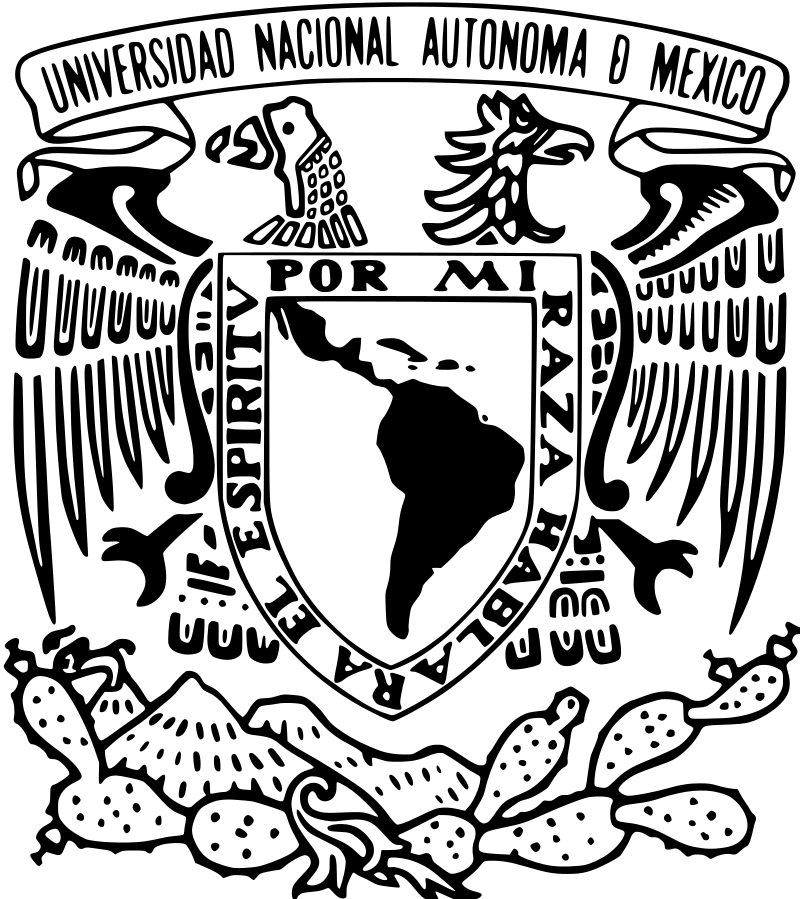
\includegraphics[width=4cm]{escudoUNAM.png}
		};

		\node[anchor=north east, inner sep=30] at (current page.north east) {
			
\includegraphics[width=4cm]{escudoFI.png}
		};
	\end{tikzpicture}

	\begin{center}
		\vspace*{3cm}

		\Huge
		\textbf{Practica 3 - Análisis Senoidal de Circuitos Trifásicos Balanceados y Desbalanceados}

		\vspace{2.5cm}

		\Huge
		\textbf{Facultad de Ingeniería}\\
		Circuitos Eléctricos\\
		Semestre 2026-1\\

		\vspace{2.5cm}

		\textbf{Grupo:} 4

		\vspace{2.5cm}

		\Huge
		Ugartechea González Luis Antonio\\
		Tepal Brinseño Hansel Yael \\
		\textbf{Fecha de entrega:}
		\vspace{2.5cm}
	\end{center}

\end{titlepage}

\section{Objetivo}

\begin{itemize}
	\item Determinar experimentalmente las relaciones entre los voltajes de línea y voltajes de fase.
	\item Determinar experimentalmente las relaciones entre las corrientes de línea y las corrientes entre líneas.
	\item Verificar la relación entre el voltaje y la corriente en un inductor.
	\item Verificar la relación entre el voltaje y la corriente en un capacitor.
	\item Mediante el empleo de un simulador electrónico de un generador trifásico balanceado analizar prácticamente un circuito trifásico, empleando fasores.
\end{itemize}

\section{Marco Teórico}

\subsection{Sistema Trifásico Balanceado}
Un sistema trifásico balanceado, o equilibrado, es un método de generación, distribución y consumo de energía eléctrica formado por tres fuentes de tensión alterna (AC) de igual magnitud y frecuencia. La característica fundamental que define a este sistema es que las tres ondas de tensión se encuentran desfasadas simétricamente entre sí por un ángulo de 120 grados eléctricos. Se considera ``balanceado'' cuando las impedancias de las cargas conectadas a cada una de las tres fases son idénticas, lo que resulta en corrientes de línea con la misma magnitud. Esta configuración es el estándar para la transmisión de energía a gran escala y para la alimentación de motores industriales debido a su eficiencia y a la entrega de potencia constante.

\subsection{Voltaje de línea}
El voltaje de línea, también conocido como tensión de línea a línea y denotado como \(V_L\) o \(V_{LL}\), es el valor de la diferencia de potencial (voltaje) medido entre dos conductores de fase cualesquiera en un sistema trifásico (e.g., entre la fase R y S, S y T, o T y R). Este es el voltaje que típicamente se especifica para la maquinaria y equipo trifásico. En una conexión tipo estrella (Y), el voltaje de línea es \(\sqrt{3}\) veces mayor que el voltaje de fase.
\( V_L = \sqrt{3} \cdot V_{\phi} \)

\subsection{Voltaje de fase}
El voltaje de fase, denotado como \(V_{\phi}\) o \(V_{LN}\), representa la diferencia de potencial medida entre un solo conductor de fase y el punto neutro (N) del sistema. Este voltaje es el que alimenta a las cargas monofásicas que se conectan a un sistema trifásico. En sistemas de distribución residenciales en algunas configuraciones, es el voltaje que llega a los enchufes convencionales.

\subsection{Corriente de línea}
La corriente de línea, denotada como \(I_L\), es la corriente eléctrica que fluye a través de cualquiera de los conductores de fase que alimentan la carga. Su valor es fundamental para el dimensionamiento de los conductores, fusibles y otros elementos de protección del sistema. La relación entre la corriente de línea y la de fase depende de la configuración de la carga.

\subsection{Corriente de fase}
La corriente de fase, denotada como \(I_{\phi}\), es la corriente que circula a través de un elemento de la carga conectado a una fase específica del sistema. Su relación con la corriente de línea varía según la conexión:
\begin{itemize}
    \item \textbf{En conexión Estrella (Y):} La corriente de línea es igual a la corriente de fase, ya que el conductor de línea alimenta directamente a la carga de fase. \(V_L = V_{\phi}\).
    \item \textbf{En conexión Delta ($\Delta$):} La corriente de línea se divide entre dos ramas de la carga, por lo que la corriente de línea es \(\sqrt{3}\) veces mayor que la corriente de fase. \(V_L = \sqrt{3} \cdot V_{\phi}\). En este tipo de circuito no hay neutro.
\end{itemize}

\subsection{Ángulo de desfasamiento}
En un sistema trifásico balanceado, el ángulo de desfasamiento es la separación angular que existe entre las ondas senoidales de tensión (o corriente) de las tres fases. Este ángulo es constante e igual a \textbf{120 grados eléctricos} (\(120^\circ\)) o \(2\pi/3\) radianes. Si se toma una fase como referencia (0\(^\circ\)), la segunda estará a 120\(^\circ\) y la tercera a 240\(^\circ\). Este desfase ordenado es lo que permite la creación de un campo magnético giratorio en los motores de inducción y asegura una entrega de potencia total mucho más suave y constante en comparación con un sistema monofásico.

\section{Desarrollo}

\subsection{Experimento 1}

\begin{figure}[H]
	\centering
	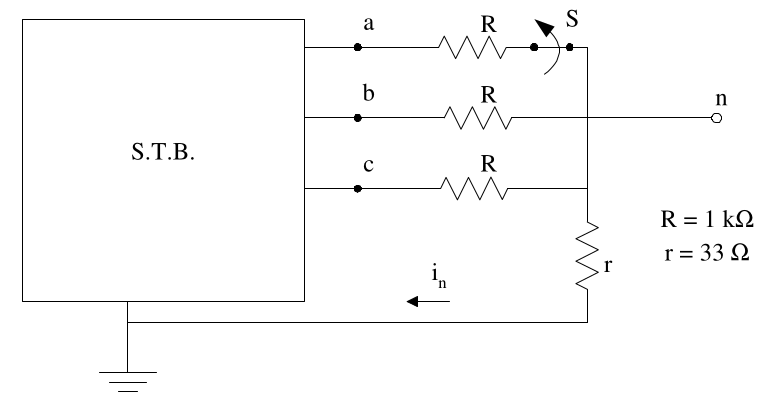
\includegraphics[width=0.6\textwidth]{circuito_exp1.png}
	\caption{Circuito del Experimento 1}
\end{figure}

\textbf{Considere:} \(V_a = 0^\circ\)

\subsubsection*{Datos del STB práctico}

\begin{itemize}
	\item \(A = 6 V\) (Voltaje de fase)
	\item \(f = 685.129 Hz\) (Frecuencia)
\end{itemize}

Del osciloscopio obtenemos el desfase entre A y B:

\[ \phi_{AB} = \frac{(125x10^{-6})(360^{\circ})}{(1.45x10^{-3})} = 31.0344^\circ \]

Y para obtener la diferencia de Voltaje utilizamos la relación:

\[ V = \left| \frac{V_{ab}}{V_{bn}} \right| = \left| \frac{10 V}{5 V} \right| = 2 [V]\]

\textbf{Nota:} Cuando desconectamos la resistencia de A cambia muy poco el voltaje de la señal de salida.

\subsection{Experimento 2}

\begin{figure}[H]
	\centering
	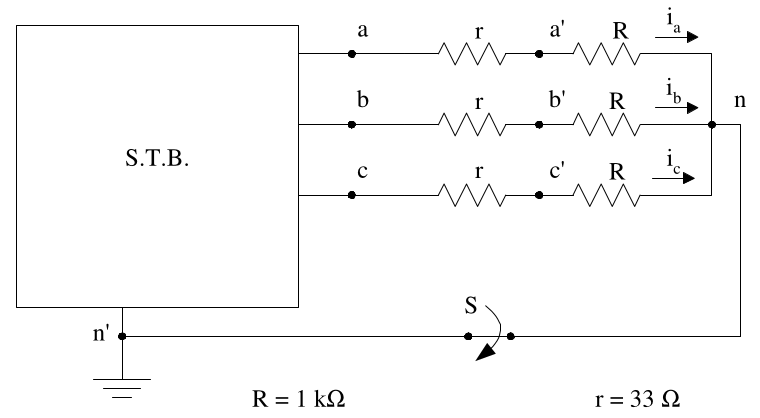
\includegraphics[width=0.6\textwidth]{circuito_exp2.png}
	\caption{Circuito del Experimento 2}
\end{figure}

% \subsection*{Datos del STB práctico}

% \begin{itemize}
% 	\item \(A = 6 V\) (Voltaje de fase)
% 	\item \(f = 685.129 Hz\) (Frecuencia)
% \end{itemize}

\subsection*{Para la corriente de línea con el switch cerrado de \(r_A\)}

\textbf{Donde:}

\begin{itemize}
	\item \(V_{L_{r_A}} = 312 [mV_p]\)
	\item \(V_{\phi_{r_A}} = 9.4 [V_p]\)
	\item \(R_{r_A} = 33 [\Omega]\)
\end{itemize}

Utilizando la ley de Ohm:

\begin{itemize}
	\item \(I_{r_A} = \frac{V_{L_{r_A}}}{R_{r_A}} = \frac{312 \times 10^{-3}}{33} = 9.4545 [mA]\)
\end{itemize}

%Para dibujar los fasores como no hay desfase uno queda encima de otro

\subsection*{Fasores para el switch cerrado}

% \begin{tikzpicture}
% 	\draw[->, thick] (0,0) -- (3,0) node[anchor=north west] {9.4 V};
% 	\draw[->, thick] (0,0) -- (0,3) node[anchor=south west] {9.4545 mA};
% \end{tikzpicture}

\subsection*{Para la corriente de línea con el switch abierto de \(r_A\)}

No varía mucho porque estamos manejando \(mV\) y al ser un sistema trifásico balanceado las corrientes son similares.

\begin{itemize}
	\item \(V_{L_{r_A}} = 312 [mV_p]\)
	\item \(V_{\phi_{r_A}} = 9.4 [V_p]\)
	\item \(R_{r_A} = 33 [\Omega]\)
\end{itemize}

Utilizando la ley de Ohm:

\begin{itemize}
	\item \(I_{r_A} = \frac{V_{L_{r_A}}}{R_{r_A}} = \frac{312 \times 10^{-3}}{33} = 9.4545 [mA]\)
\end{itemize}

\subsection*{Fasores para el switch abierto}

% \begin{tikzpicture}
% 	\draw[->, thick] (0,0) -- (3,0) node[anchor=north west] {9.4 V};
% 	\draw[->, thick] (0,0) -- (0,3) node[anchor=south west] {9.4545 mA};
% \end{tikzpicture}

\subsection*{Análisis de resultados}

Como se puede observar en las mediciones realizadas, los valores de voltaje y corriente se mantienen prácticamente constantes tanto con el switch cerrado como abierto. Esta estabilidad en las mediciones confirma las características fundamentales de un sistema trifásico balanceado:

\begin{itemize}
	\item La corriente de línea permanece en 9.4545 mA independientemente del estado del switch
	\item El voltaje de fase se mantiene estable en 9.4 V
	\item La variación mínima observada es atribuible a la precisión de los instrumentos de medición
\end{itemize}

Este comportamiento valida la teoría de que en un sistema trifásico balanceado, la desconexión de una carga no afecta significativamente las condiciones de operación de las otras fases, debido a la simetría del sistema y la distribución equilibrada de las cargas.

\subsection{Experimento 3}

\begin{figure}[H]
	\centering
	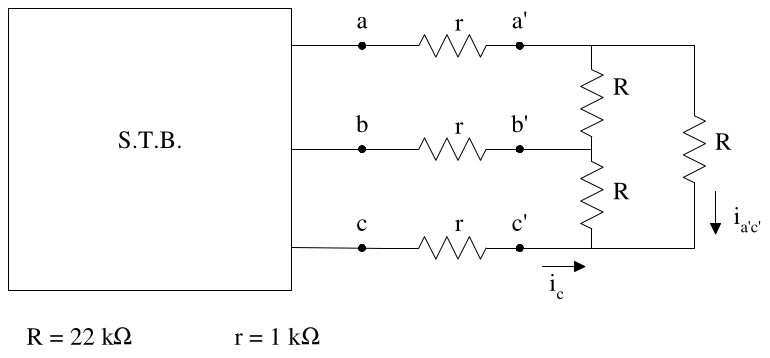
\includegraphics[width=0.6\textwidth]{circuito_exp3.png}
	\caption{Circuito del Experimento 3}
\end{figure}

\subsubsection*{Ángulo de desfase práctico}

\[\phi = 30.3^\circ \]

\subsubsection*{Voltaje de línea práctico}

\[ V_{L_{r_C}} = 1.36 V \]

\[ V_{L_{a'-c'}} = 15.6 V \]


\subsubsection*{Para la corriente \(I_{c}\) y \(I_{a'-c'}\)}

\textbf{Donde:}

\begin{itemize}
	\item \(V_{L_{r_C}} = 1.36 [V_p]\)
	\item \(V_{L_{a'-c'}} = 15.6 [V_p]\)
	\item \(R = 22 [k\Omega]\)
	\item \(r = 1 [k\Omega]\)
\end{itemize}



% \subsection{Experimento 4}

% \begin{figure}[H]
% 	\centering
% 	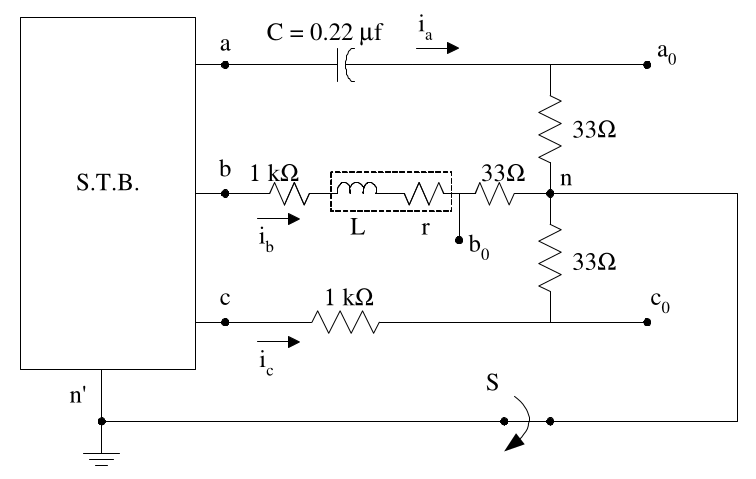
\includegraphics[width=0.6\textwidth]{circuito_exp4.png}
% 	\caption{Circuito del Experimento 4}
% \end{figure}

\section{Conclusiones}

% \section{Bibliography}

% \begin{biblio}
% 	%for: https://www.poli.edu.co/blog/poliverso/diseno-digital-que-es
% 	\item \textit{Diseño digital: qué es y por qué es importante.} (2021, August 26). Poliverso. Retrieved October 16, 2024, from: \textcolor{blue}{\underline{\url{https://www.poli.edu.co/blog/poliverso/diseno-digital-que-es}}}
% 	%for: https://www.sky6cancun.com/marketing/diseno-grafico/diseno-digital-que-es-y-para-que-sirve/
% 	\item \textit{Diseño digital: qué es y para qué sirve.} (2021, August 26). Sky6Cancún. Retrieved October 16, 2024, from: \textcolor{blue}{\underline{\url{https://www.sky6cancun.com/marketing/diseno-grafico/}}}
% \end{biblio}

\end{document}
